


\section{Relevant text detection}
\label{cp4:corpus-relevant-text}


%Provided that we have a set of software tasks and pertinent artifacts associated with each task, 
%the last step in our corpus creation pipeline is the detection of relevant information within 
%each pertinent artifact. 
\gm{Next, we need to identify relevant
text for the task in selected
artifacts for the task.}

\gm{I think you need to set up
that you want the state-of-the-art
because you want to do at least
this good with your newly developed
techniques that motivates the creation
of this corpus in the first place.
You'll also have to explain the
Misc ones.}

To that end, we rely on state-of-the-art approaches able to automatically identify relevant text for the tasks and artifacts in our corpus~\cite{nadi2020, Robillard2015, Lotufo2012, Xu2017}.


To identify techniques applicable to the creation of our corpus, we systematically reviewed related work. We searched for techniques based on their availability in existing replication packages and their readiness for use.
We also refrained from using approaches with training procedures (e.g., ~\cite{liu2020} or ~\cite{Treude2016}) because of the challenges related to correctly tuning such supervised approaches~\cite{Chaparro2017, fucci2019}. Based on these criteria, three techniques were selected for the artifact sources in parenthesis:


\begin{itemize}[leftmargin=\parindent, font=\normalfont\itshape]
    \item \texttt{\acs{AnsBot}} (\textit{SO Answers}) uses several features (e.g., information entropy, textual patterns, entity overlap, etc.) to determine that a sentence has useful information to a developer's technical question~\cite{Xu2017}.
    
    \item \texttt{\acs{Krec}} (\textit{API Documentation}) identifies text fragments that reflect ``potentially important text that programmers cannot afford to ignore when using the API''~\cite{Robillard2015}.
    
    \item \texttt{\acs{Hurried}} (\textit{GitHub issues}) identify the most relevant sentences in a bug report based on three factors used to assess a sentence's relevancy (i.e., sentence's prominence in the issue, topic, and its similarity to the task)~\cite{Lotufo2012}.
\end{itemize}



While our corpus also has miscellaneous Web pages (i.e., Web tutorials or blog posts), we are not aware of a technique able to identify task-relevant text for such sources. We detail how we make use of miscellaneous sources in Section~\ref{}.

\gm{I think you have to be clearer  that
Misc are included as non-annotated artifacts.}



For the pertinent artifacts of our running example (Figure~\ref{fig:lock-screen-task}), 
Tables~\ref{tbl:git-example-ansbot} to~\ref{tbl:git-example-hurried}
illustrate sentences automatically detected by \acs{AnsBot}, \acs{Krec}, and \acs{Hurried}, respectively.
\gm{Why give these three examples?}
 


\begin{table}[H]
\centering    
\begin{scriptsize}
\begin{threeparttable}
\rowcolors{2}{}{lightgray}
\begin{tabular}{ll}

\hline
\multicolumn{2}{c}{\textit{How to add MediaPlayer controls on lock screen?}} \\
\hline
\hline

1 & \parbox[l][.8cm][c]{10.5cm}{I had the same problem, and well, the solution was simple, do not use any widget, simply use the RemoteControlClientCompat class.} \\
2 & \parbox[l][.8cm][c]{10.5cm}{Here is my lockScreenControls() method code, which I call whenever I want to show this type of control (when plays a song).} \\
3 & \parbox[l][.5cm][c]{10.5cm}{Thank @ianhlake for the good 2 video} \\

\hline


\end{tabular}
\end{threeparttable}
\end{scriptsize}
\caption{Pertinent sentences automatically detected by \acs{AnsBot}}
\label{tbl:git-example-ansbot}
\end{table}

\begin{table}[H]
\centering    
\begin{scriptsize}
\begin{threeparttable}
\rowcolors{2}{}{lightgray}
\begin{tabular}{ll}
    
\hline
\multicolumn{2}{c}{\textit{Lock task mode - Android Developers}} \\
\hline
\hline

1 & \parbox[l][.8cm][c]{10.5cm}{You might use lock task mode if you're developing a kiosk application or a launcher to present a collection of apps.} \\
2 & \parbox[l][.8cm][c]{10.5cm}{To check if the current app is running in lock task mode, use the methods on ActivityManager as shown in the following example:} \\
3 & \parbox[l][.8cm][c]{10.5cm}{You can call KeyguardManager methods to find out if the device is locked and use an Activity lifecycle callback (such as onResume() that's called after unlocking) to start lock task mode.} \\
\hline

\end{tabular}
\end{threeparttable}
\end{scriptsize}
\caption{Pertinent sentences automatically detected by \acs{Krec}}
\label{tbl:git-example-krec}
\end{table}

\begin{table}[H]
\centering    
\begin{scriptsize}
\begin{threeparttable}
\rowcolors{2}{}{lightgray}
\begin{tabular}{ll}

\hline
\multicolumn{2}{c}{\textit{How to add MediaPlayer controls on lock screen?}} \\
\hline
\hline

1 & \parbox[l][.8cm][c]{10.5cm}{I had the same problem, and well, the solution was simple, do not use any widget, simply use the RemoteControlClientCompat class.} \\
2 & \parbox[l][.8cm][c]{10.5cm}{Here is my lockScreenControls() method code, which I call whenever I want to show this type of control (when plays a song).} \\
3 & \parbox[l][.5cm][c]{10.5cm}{Thank @ianhlake for the good 2 video} \\

\hline


\end{tabular}
\end{threeparttable}
\end{scriptsize}
\caption{Pertinent sentences automatically detected by \acs{Hurried}}
\label{tbl:git-example-hurried}
\end{table}







\subsection{Ratio of Task-relevant Sentences}
\label{cp4:corpus-relevant-text-ratio}

\gm{You need to get across that in applying
the techniques to this new data you need to
check if the results are similar to what was
reported for the technique authors. Doesn't
this require you to speak to whether the accuracy
is similar to what the authors reported for
the techniques?}

\gm{W}e apply a set of techniques 
to tasks/artifacts outside the ones where the techniques were originally proposed and evaluated~\cite{nadi2020, Robillard2015, Lotufo2012, Xu2017}.
For instance, \acs{AnsBot}'s design was based on general Java programming tasks~\cite{Xu2017} while the tasks in our corpus comprise Android development and originate both from GitHub and from Stack Overflow. Because of such differences, we ask:


\begin{enumerate}[label={},leftmargin=0.7cm]
\item \textit{Within the artifacts in our corpus, what is the average ratio of sentences relevant to a task detected by the selected techniques?} 

\end{enumerate}



Answering this question will assist in defining \textit{thresholds} or the \textit{ratio}
of the text in each artifact that our selected techniques identify as useful to a particular task.
In turn, this information will allow us to use the \acs{DS-android} corpus for the design and evaluation of techniques that we later propose (Chapter~\ref{ch:identifying}).



To answer this question, we rely on three reference answers produced by 
experienced software developers to define \textit{golden relevant sentences} 
and to compute ratios for a sample of 10 tasks and associated artifacts in our corpus.
The following subsections provide further details on how we compute ratios.

\art{I used `ratio' to move away from `evaluation'. Accuracy can be better, but just thinking if it still implies an evaluation. Does it?}





\subsubsection{Golden Data}


Creating golden data for the entirety of the \acs{DS-android} corpus is infeasible
since it would require asking human evaluators to inspect thousands of artifacts and more than 260,000 sentences.
Due to this reason, we restrict computing ratios to a random subset of 10 tasks in our corpus (i.e., 5 GitHub tasks and 5 Stack Overflow tasks). 
From now on, we refer to this subset as the \textbf{\acs{DS-android-small}} corpus.


For each one of the tasks in the \acs{DS-android-small} corpus, we also randomly selected 
one artifact for each of the techniques we intend to use, i.e., one API document, a Github issue discussion, one Stack Overflow answer, as well as two randomly selected miscellaneous artifacts for a maximum of 5 artifacts per task.

\gm{Are you not having the annotators do all artifacts?
Isn't it only 50? If you only have three annotators otherwise you don't get enough data?}

%  TODO: update this once I review the web tutorials/blogs
% Overall, this corpus has 2,375 sentences with an average of 64 sentences per artifact---
% a size comparable to the \acs{DS-synthetic} corpus~\cite{marques2020}.
% ($\mypm$ 72)

\gm{There is no evaluation, so use annotators not
evaluators}

We asked human evaluators to read the content of these
artifacts and 
to mark sentences that they deemed useful and that provide information that assisted task completion---instructions similar to the ones used for the creation of the 
data in the \acs{DS-synthetic} corpus~\cite{marques2020}.
Since individuals might use different criteria to
assess relevance~\cite{Barry1994, Barry1998, Freund2015},
there is a risk that
the text selected by annotators does not overlap~\cite{Freund2013, Freund2015}.
Due to this reason, golden data in \acs{DS-android-small} consists of any sentence marked by evaluators. 

% Section~\ref{cp4:threats} further details threats that might arise from this decision.



% Additionally, the text selected by a single annotator may still be crucial for task completion~\cite{marques2020}.


\subsubsection{Annotators}
\textcolor{white}{force ident} % this is just for the chapter outline

--- We recruited \red{n} graduate students with professional programming experience to produce \textit{golden} data for our tasks sample. \vspace{3mm}


\subsubsection{Annotation Procedures}

\gm{golden data, rather than goldens}

Our intention is that goldens reflect text that an experienced developer would deem as useful for task completion and that they would share with someone eager to make their \textit{first contribution} in an open-source project.

\gm{Is this goal consistent with what the
original techniques sought to do as well?}

\gm{Doesn't each annotator get each of the 10
tasks so there is no randomly assigned task?}

To produce such data, annotators had at their disposal a set of randomly assigned task descriptions and links to artifacts pertinent to the respective task. We asked annotators to write a short plan (250 words max~\cite{Rastkar2010}) with instructions that a newcomer could follow to successfully complete the task. 
The purpose of the plan was to ensure that annotators built enough context about the task.
While perusing artifacts, annotators also had to manually highlight sentences that they deemed useful and that provided information that assisted task completion. 


The annotation process was facilitated by an in-house tool---in the form of a Web browser plugin shown in Figure~\ref{fig:corpus-annotation-tool}. In the figure, the top-right corner panel shows the browser extension. Annotators could start an annotation session and click the highlight button.
This would instrument the HTML of a page and identify each sentence in a paragraph. The tool allowed annotators to hove over individual sentences and select them as relevant (text in orange) by clicking on the hovered text. For example, the figure depicts that an annotator selected  the sentence
``\textit{Call {\small \texttt{ActivityOptions.setLockTaskEnabled()}} ... when starting the activity}'' as relevant for the lock mode task.


\begin{figure}
    \centering
    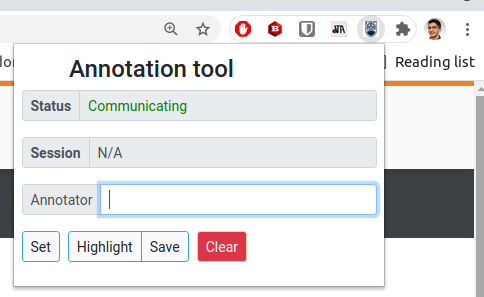
\includegraphics[width=\textwidth]{cp4/annotation-tool}
    \caption{Annotation tool and relevant sentences marked by an annotator}
    \label{fig:corpus-annotation-tool}
\end{figure}



\subsection{Metrics}


Based on the golden data, we use a sliding scale to determine the ratio of task-relevant text identified by each technique. That is, we compute ratios considering when one, two or the three annotators have marked a sentence as relevant.


We  
compute the ratio of sentences identified by a technique using standard \textit{precision} and \textit{recall} metrics~\cite{Manning2009IR}. When computing metrics, we compare the relevant text automatically identified by a technique against the golden relevant text 
selected by a given number of annotators (i.e., $n=1, 2,$ or $3$)

\gm{I am not quite following ratio here...}



To ease interpreting precision and recall, Table~\ref{tbl:type-I-II-errors} show all possible evaluation outcomes. The \textit{relevant} and \textit{not-relevant} columns represent the text 
marked (or not) by the annotators. Rows represent the text automatically identified by a technique.




 


\begin{table}[H]
\centering    
\begin{scriptsize}
\begin{threeparttable}
\begin{tabular}{l|l|l}

\hline

\textbf{}
& \textbf{Relevant}    
& \textbf{Not-relevant} \\

\hline
\hline

\textbf{Identified as relevant} & true positive ($TP$) & false positive ($FP$) \\
\hline
\textbf{Identified as Not-relevant} & false negative ($FN$) & true negative ($TN$) \\
\hline

\end{tabular}
\end{threeparttable}
\end{scriptsize}
\caption{Result outcomes}
\label{tbl:type-I-II-errors}
\end{table}

    



For a given task $t$ and artifact $a$, $precision_n$ is the ratio between the sentences identified that are marked as relevant by $n$ annotators and the total number of sentences identified, as shown in Equation~\ref{eq:cp4:precision}. For example,  \textit{precision(t, API documentation)\textsubscript{2}} computes the number of sentences identified by \acs{Krec} for the task $t$ when 
goldens consist of sentences marked by two or more annotators.


\begin{equation}
\label{eq:cp4:precision}    
    Precision(t, a)_n = \frac{TP}{TP + FP}
\end{equation}


Recall ($recall_n$) represents how many of all sentences marked by at least $n$ annotators are identified by a technique (Equation~\ref{eq:cp4:recall}).



\begin{equation}
\label{eq:cp4:recall}        
    Recall(t, a)_n = \frac{TP}{TP + FN}
\end{equation}

\vspace{3mm}




\subsection{Results}
\textcolor{white}{force ident} % this is just for the chapter outline


--- Discuss results.\footnote{\red{think which summary tables should I have in the thesis body and which I can move to Appendices}} \vspace{3mm}



--- Precision~\ref{tbl:ds-small-results-precision}  \vspace{3mm}


--- Recall~\ref{tbl:ds-small-results-recall} \vspace{3mm}

--- Likely explanation for the results obtained.

% When interpreting results, we favor precision instead of recall.
% A false positives may contribute to a developer abandoning reading of an artifact that would otherwise provide crucial information for her task~\cite{Rastkar2010}.




\begin{table}[H]
\centering    
\begin{scriptsize}
\begin{threeparttable}
\begin{tabular}{lcccccc}

\hline


\multirow{2.5}{*}{Technique}
& \multicolumn{2}{c}{\textit{$Precision_{n=3}$}}
& \multicolumn{2}{c}{\textit{$Precision_{n=2}$}}
& \multicolumn{2}{c}{\textit{$Precision_{n=1}$}}
\\ \cmidrule(l){2-3} \cmidrule(l){4-5} \cmidrule(l){6-7} 


& \textit{mean}
& \textit{std}
& \textit{mean}
& \textit{std}
& \textit{mean}
& \textit{std}
\\


\hline
\hline

\acs{AnsBot} 
& 0.5 & 0.5 % = 3
& 0.5 & 0.5 % = 2
& 0.5 & 0.5 % = 1
\\

\acs{Krec} 
& 0.5 & 0.5 % = 3
& 0.5 & 0.5 % = 2
& 0.5 & 0.5 % = 1
\\

\acs{Hurried} 
& 0.5 & 0.5 % = 3
& 0.5 & 0.5 % = 2
& 0.5 & 0.5 % = 1
\\

\hline

\end{tabular}
\end{threeparttable}
\end{scriptsize}
\caption{Precision of each technique for the tasks of \acs{DS-android-small}}
\label{tbl:ds-small-results-precision}
\end{table}

    

% \begin{table}[H]
% \centering    
% \begin{scriptsize}
% \begin{threeparttable}
% \begin{tabular}{lcccccccccccc}

% \hline


% \multirow{2.5}{*}{Technique}
% & \multicolumn{10}{c}{\textit{Tasks}} 
% & \multicolumn{2}{c}{\textit{Precision}}
% \\  \cmidrule(l){2-11} \cmidrule(l){12-13} 



% &
% \textit{T1} & \textit{T2} & \textit{T3} & \textit{T4} & \textit{T5}
% & \textit{T6} & \textit{T7} & \textit{T8} & \textit{T9} & \textit{T10}
% & \textit{mean}
% & \textit{std}
% \\


% \hline
% \hline

% \acs{AnsBot} 
% & 0.5 & 0.5 & 0.5 & 0.5 & 0.5
% & 0.5 & 0.5 & 0.5 & 0.5 & 0.5
% & 0.5 % mean
% & 0.5 % std
% \\

% \acs{Krec} 
% & 0.5 & 0.5 & 0.5 & 0.5 & 0.5
% & 0.5 & 0.5 & 0.5 & 0.5 & 0.5
% & 0.5 % mean
% & 0.5 % std
% \\

% \acs{Hurried} 
% & 0.5 & 0.5 & 0.5 & 0.5 & 0.5
% & 0.5 & 0.5 & 0.5 & 0.5 & 0.5
% & 0.5 % mean
% & 0.5 % std
% \\

% \hline

% \end{tabular}
% \end{threeparttable}
% \end{scriptsize}
% \caption{Precision of each technique for the tasks of \acs{DS-android-small}}
% \label{tbl:ds-small-results-precision}
% \end{table}

    

\begin{table}[H]
\centering    
\begin{scriptsize}
\begin{threeparttable}
\begin{tabular}{lcccccc}

\hline


\multirow{2.5}{*}{Technique}
& \multicolumn{2}{c}{\textit{$Recall_{n=3}$}}
& \multicolumn{2}{c}{\textit{$Recall_{n=2}$}}
& \multicolumn{2}{c}{\textit{$Recall_{n=1}$}}
\\ \cmidrule(l){2-3} \cmidrule(l){4-5} \cmidrule(l){6-7} 


& \textit{mean}
& \textit{std}
& \textit{mean}
& \textit{std}
& \textit{mean}
& \textit{std}
\\


\hline
\hline

\acs{AnsBot} 
& 0.5 & 0.5 % = 3
& 0.5 & 0.5 % = 2
& 0.5 & 0.5 % = 1
\\

\acs{Krec} 
& 0.5 & 0.5 % = 3
& 0.5 & 0.5 % = 2
& 0.5 & 0.5 % = 1
\\

\acs{Hurried} 
& 0.5 & 0.5 % = 3
& 0.5 & 0.5 % = 2
& 0.5 & 0.5 % = 1
\\

\hline

\end{tabular}
\end{threeparttable}
\end{scriptsize}
\caption{Recall of each technique for the tasks of \acs{DS-android-small}}
\label{tbl:ds-small-results-recall}
\end{table}

    


\subsection{Threats}
\label{cp4:corpus-threats}

--- \red{Argue that this is not a replication study but rather establishing thresholds} \vspace{3mm}

--- Discuss threats \vspace{3mm}



